\documentclass[t]{beamer}
\mode<presentation>

\usepackage{etex}

\usetheme{Madrid}
% other themes: Warsaw, AnnArbor, Antibes, Bergen, Berkeley, Berlin, Boadilla, boxes, CambridgeUS, Copenhagen, Darmstadt, default, Dresden, Frankfurt, Goettingen,
% Hannover, Ilmenau, JuanLesPins, Luebeck, Madrid, Maloe, Marburg, Montpellier, PaloAlto, Pittsburg, Rochester, Singapore, Szeged, classic

\setbeamertemplate{navigation symbols}{\insertslidenavigationsymbol}

\usecolortheme{dolphin}
%\usecolortheme{seagull}
% color themes: albatross, beaver, beetle, crane, default, dolphin, dov, fly, lily, orchid, rose, seagull, seahorse, sidebartab, structure, whale, wolverine

%\usefonttheme{serif}
% font themes: default, professionalfonts, serif, structurebold, structureitalicserif, structuresmallcapsserif

% pdf is displayed in full screen mode automatically
%\hypersetup{pdfpagemode=FullScreen}

%\AtBeginSection[]
%{
%  \begin{frame}<beamer>
%    \frametitle{Outline}
%    \tableofcontents[currentsection,currentsubsection]
%  \end{frame}
%}

% define your own colours:
\definecolor{Red}{rgb}{1,0,0}
\definecolor{Blue}{rgb}{0,0,1}
\definecolor{Green}{rgb}{0,1,0}
\definecolor{magenta}{rgb}{1,0,.6}
\definecolor{lightblue}{rgb}{0,.8,1}
\definecolor{lightpurple}{rgb}{.6,.4,1}
\definecolor{gold}{rgb}{.6,.5,0}
\definecolor{orange}{rgb}{1,0.4,0}
\definecolor{hotpink}{rgb}{1,0,0.5}
\definecolor{newcolor2}{rgb}{.5,.3,.5}
\definecolor{newcolor}{rgb}{0,.3,1}
\definecolor{newcolor3}{rgb}{1,0,.35}
\definecolor{darkgreen1}{rgb}{0, .35, 0}
\definecolor{darkgreen}{rgb}{0, .6, 0}
\definecolor{darkred}{rgb}{.75,0,0}

\xdefinecolor{olive}{cmyk}{0.64,0,0.95,0.4}
\xdefinecolor{purpleish}{cmyk}{0.75,0.75,0,0}

%\usepackage{beamerinnerthemerounded}
% inner themes include circles, default, inmargin, rectangles, rounded

%\usepackage{beamerouterthemesmoothbars}
% outer themes include default, infolines, miniframes, shadow, sidebar, smoothbars, smoothtree, split, tree

\useoutertheme[subsection=false]{smoothbars}

% to have the same footer on all slides
\setbeamertemplate{footline}[text line]{
\raisebox{3pt}{
\includegraphics[height=15pt]{su-long.eps}}\hfill 
\raisebox{5pt}{Math 207:  Statistics}\hfill 
\raisebox{5pt}{Chapter 6: Measurement Error}\hfill
\raisebox{5pt}{\insertframenumber/\pageref{lastpage}}}
%\setbeamertemplate{footline}[text line]{} % or empty footer

% include packages
\usepackage{subfigure}
\usepackage{multicol}
\usepackage{amsmath}
\usepackage{epsfig}
\usepackage{graphicx}
\usepackage[all,knot]{xy}
\xyoption{arc}
\usepackage{url}
\usepackage{multimedia}
\usepackage{hyperref}
\usepackage{setspace}

\title{Math 207:  Statistics}
\subtitle{Chapter 6:  Measurement Error}
\author{Ralph Wojtowicz}
\institute{Mathematics Department\\ Shenandoah University}
%\date{\scriptsize 30 January 2012}

\usepackage{pstricks,pst-grad,pst-func,pst-text,pst-node,multido,pst-plot,calc,pst-3dplot}

\newcommand{\BRACE}{
\begin{pspicture}(-3,-2.1)(3,1.1)
\psset{yunit=3,linewidth=0.02}
\psline(-3.5,0)(3.5,0)  
  \psline(-3,0)(-3,-0.04) \rput[t](-3,-0.07){\scriptsize -3\hphantom{-}}
  \psline(-2,0)(-2,-0.04) \rput[t](-2,-0.07){\scriptsize -2\hphantom{-}}
  \psline(-1,0)(-1,-0.04) \rput[t](-1,-0.07){\scriptsize -1\hphantom{-}}
  \psline(0,0)(0,-0.04)   \rput[t](0,-0.07){\scriptsize 0}
  \psline(1,0)(1,-0.04)   \rput[t](1,-0.07){\scriptsize 1}
  \psline(2,0)(2,-0.04)   \rput[t](2,-0.07){\scriptsize 2}
  \psline(3,0)(3,-0.04)   \rput[t](3,-0.07){\scriptsize 3}
  \rput[l](3.6,0){\scriptsize $x$}
\psline(0,0)(0,0.5)
  \psline(-0.12,0.5)(0,0.5)    \rput[r](-0.21,0.5){\scriptsize $0.5$}
  \psline(-0.12,0.25)(0,0.25)  \rput[r](-0.21,0.25){\scriptsize $0.25$}
\psGauss[linecolor=blue,linewidth=0.02,sigma=1,mue=0]{-3}{3}
\pnode(-1,-0.15){A}\pnode(1,-0.15){B}
\psbrace[braceWidth=0.02,braceWidthInner=5pt,braceWidthOuter=5pt](A)(B){\rput{90}(0.25,-0.05){\scriptsize 68\%}}
%
\pnode(-2,-0.15){C}\pnode(2,-0.15){D}
\psbrace[braceWidth=0.02,braceWidthInner=25pt,braceWidthOuter=5pt](C)(D){\rput{90}(0.25,-0.05){\scriptsize 95\%}}
%
\pnode(-3,-0.15){E}\pnode(3,-0.15){F}
\psbrace[braceWidth=0.02,braceWidthInner=45pt,braceWidthOuter=5pt](E)(F){\rput{90}(0.25,-0.1){\scriptsize 99.7\%}}
\end{pspicture}}

\begin{document}

%\frame[plain]{
%	\titlepage
%}


\begin{frame}[plain]
\definecolor{myblue}{rgb}{0,0,0.6}
\definecolor{grayA}{rgb}{0.95,0.95,0.95}
\definecolor{grayB}{rgb}{0.98,0.98,0.98}
\begin{center}

%\begin{pspicture}(0,0)(7,4.8)
\begin{pspicture}(-6,-7)(6,2)
\rput(0,-1.85){\scalebox{0.95}{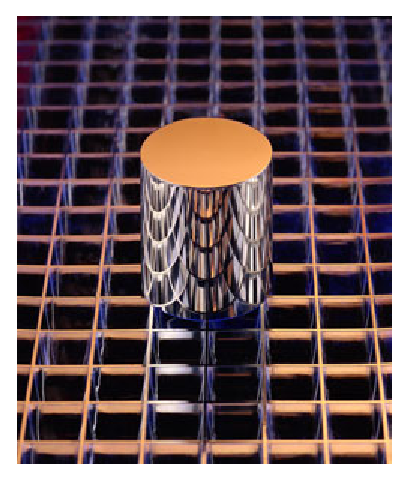
\includegraphics[height=1.7in]{KG.eps}}}
\psframe[linewidth=0.02,linecolor=gray](-6.2,-7)(6.2,2.2)
\psframe[linewidth=0.02,linecolor=gray](-6.15,-6.95)(6.15,2.15)
\rput(0,1.4){\color{myblue}\large Math 207:  Statistics}
\rput(0,0.6){\color{myblue}Chapter 6:  Measurement Error}
%\psframebox(0,0)(4,4)
\rput(0,-4.4){\scriptsize Dr.~Ralph Wojtowicz}
\rput(0,-4.9){\scriptsize Mathematics Department}
\rput(0,-5.8){
\includegraphics[height=1cm]{su-long.eps}}
%
%\rput(0,-6.5){\scriptsize 30 January 2012}
\end{pspicture}
\end{center}

\end{frame}

%\section[Outline]{}

\addtocounter{page}{-1}
\addtocounter{framenumber}{-1}

{\footnotesize
\frame{\tableofcontents}
}

\section{Introduction}
\subsection{Introduction}
\begin{frame}[t]\frametitle{Introduction}
{\small
\begin{itemize}
\item In the real world, if we measure something several times, we observe
  different values each time.
\item Each result is thrown off by {\color{blue}chance error}.
\item How do these errors arise? 
\item How big are they likely to be? (Chapter 6)
\item How much is likely to cancel out in the average? (Chapters 20--21, 23--24)
\\ Standard error:  SE (for sum, average or percent)
\end{itemize}}

\end{frame}

\section{Chance Error}
\subsection{Chance Error}
\begin{frame}[t]\frametitle{Chance Error}
{\small
\begin{itemize}
\item Standards weights are maintained at local, state, national 
  and international levels for commercial, scientific and other purposes.
\item The International Bureau of Weights and Measures near Paris
  maintains the International Prototype Kilogram.
\item The National Bureau of Standards in Washington, D.C. 
  maintains a national prototype kilogram (Kilogram \#20) 
  that is calibrated against
  the international standard.
\item The Bureau maintains several other standard weights that are
  calibrated against Kilogram \#20.
\item NB 10 is one such standard weight.  It weighs very nearly 10 grams.
\item Our text has a table of 100 measurements of NB 10.
\end{itemize} 
}
\end{frame}

\subsection{NB 10}
\begin{frame}[t]\frametitle{NB 10}
\newcommand{\HH}{\hspace{20pt}}
\newcommand{\HP}{\hphantom{9.999}}
{\small
\begin{itemize}
\item NB 10 is a 10 gram weight maintained by the National 
  Bureau of Standards.
\item The first five NB 10 measurements (in grams) from Table 1 on page 99
  are:
\vspace{-5pt}
\end{itemize}
\[9.999591\HH 9.999600\HH 9.999594\HH 9.999601\HH 9.999598\]\vspace{-15pt}
\begin{itemize}
\item Measurements are in terms of micrograms below 10 grams:\vspace{-3pt}
\end{itemize}
\[\HP409\HH \HP400\HH \HP406\HH \HP399\HH \HP402\]\vspace{-17pt}
\begin{itemize}
\item For the measurements in Table 1, 
  $\mbox{mean}\approx 405$
 and $\mbox{SD}\approx 6$ in micrograms.
\end{itemize}
}
\end{frame}

\subsection{NB 10 Data Exercises}
\begin{frame}[t]\frametitle{NB 10 Data Exercises}
{\small
\begin{itemize}
\item Use the following to load the data into \texttt{R}:\\[2pt]
{\scriptsize  \texttt{> nb10 <- read.table("http://www.adjoint-functors.net/su/web/314/R/NB10")}}
\item  Use \texttt{R} to compute the mean, SD, max, min, and
 quantiles (using \texttt{summary(nb10)}).
\item Compare the median (use the quantiles or
   \texttt{median(nb10\$V1)}) to the mean.
\item Plot a histogram of the data.  
   Does it look like the normal curve?\\[2pt]
    \texttt{> hist(nb10\$V1, probability=TRUE, breaks=40)}
\item Calculate the fraction of the data within 1 SD of the mean.\\
   \texttt{> m <- mean(nb10\$V1)}\\
   \texttt{> s <- SD(nb10\$V1)}\\
   \texttt{> length(nb10\$V1[m-s < nb10\$V1 \&  nb10\$V1 < m+s])}
\item   What fraction of the data is within 2 SDs of the mean?  3 SDs?
   4?  5? 6?
   How do these percentages compare to those of the normal curve?
\item Compare \texttt{SD(nb10)} to \texttt{sd(nb10)}.  Why are 
  the values so close?
\end{itemize}
}
\end{frame}

\section{Outliers}
\subsection{Outliers}
\begin{frame}[t]\frametitle{Outliers}
\newcommand{\U}{\underline{\hspace{5pt}}}
{\begin{itemize}
\item The NB 10 data does not fit the normal curve very well.
   The data is a bit more crowded around the mean than it should be.
   Value \#36 is 3 SDs from the mean and \#86 and \#94 
    are 5 SDs away.\\
  \begin{itemize}
  \item Run the following test:  \texttt{shapiro.test(nb10\$V1)}.\\
         The $p$-value reported by the Shapiro test answers the following question:  
         If the measurement process has a normal distribution, what is the probability
         of getting the observed data?  What was the $p$-value that your test calculated
    and what does it mean?
  \item Try the following:
    \texttt{shapiro.test(rnorm(100, mean=0, sd=5))}.  Repeat this several times. What do the 
    results tell you?
%    How many data values are in this new list?
  \end{itemize}
\item Repeat the exercises from the previous slide using the file\\
{\scriptsize  \texttt{http://www.adjoint-functors.net/su/web/314/R/NB10\U noOutliers}}\\
\item This data fits the normal curve better.
\item Should the outliers be discarded?  No.  See page 103.\\[10pt]
%\item \textbf{Computer exercises}:  
%   \begin{itemize}
%    \item Write out solutions to the  exercises on this and the 
%      previous slide.  
%    \item Work in groups of 2--3 students (no individual assignments will be graded).
%    \item Please write sentences to explain and discuss your answers.
%       Use this as an opportunity to study for Exam 1 (Friday 10 January).
%    \item Due Friday, 10 January 
%    \end{itemize}
\end{itemize}
}
\end{frame}


\section{Bias}
\subsection{Bias}
\begin{frame}[t]\frametitle{Bias}
{\small
\begin{itemize}
\item {\color{blue}Bias} affects all measurements the same way, pushing
  them in the same direction.
\item {\color{blue}Chance errors} change from measurement to measurement,
  sometimes up and sometimes down.\vspace{-3pt}
\end{itemize}
\[\mbox{(individual measurement)} = \mbox{(exact value)}\, +\, \mbox{bias}
  \, +\,
   \mbox{(chance error)}\vspace{-10pt}\]
\begin{itemize}
\item If there is no bias, the long-run average of repeated measurements 
  should approach the exact value.
 Chance errors should cancel out in the average.
\end{itemize}
}
\label{lastpage}
\end{frame}


\end{document}
